\subsection{Adjustment stage}

MultiGWAS takes as input a configuration file where the user specifies the genomics data and the parameters used by the four tools. Once the configuration file is read and processed, the genomic data files (genotype and phenotype) are then cleaned, filtered, and checked for data quality. The output of this stage corresponds to the inputs for the four programs at the Multi Analysis stage.

%genotype/phenotype filenames, genome-wide significance threshold, multiple testing correction methods, GWAS model, number of associations to be reported, and TRUE or FALSE whether to use quality control (QC) filters or not. 

\subsubsection{Reading configuration file\label{section-Reading-configuration-file}}

The configuration file includes the following settings that we briefly describe:% (1) Input genotype and phenotype file names (2) GWAS model, (3) Significance threshold, (4) Correction (5) Quality Control (QC) filters and (6) number of associations to report. 

\paragraph{{Ploidy:}} Numerical value for the ploidy level of the genotype, currently MultiGWAS supports diploids and tetraploids genotypes (2: for diploids, 4: for tetraploids).

\paragraph{{Genotype and phenotype input files:}}

MultiGWAS uses two input files, one for the genotype and one for the phenotype. Genotypes files can be either in GWASpoly format (\cite{Rosyara2016}) using SNP markers in rows and samples in columns (Fig. \ref{fig:File-Formats}.a) or Variant Call Format (VCF) (Fig.\ref{fig:File-Formats}.b) which is transformed into GWASpoly format using NGSEP 4.0.2 (\cite{Duitama2019}). The phenotype file contains only one trait and uses a matrix format with the first column for the sample names and the second column for the trait values (Fig. \ref{fig:File-Formats}.c).

\begin{figure}[H]
\begin{centering}
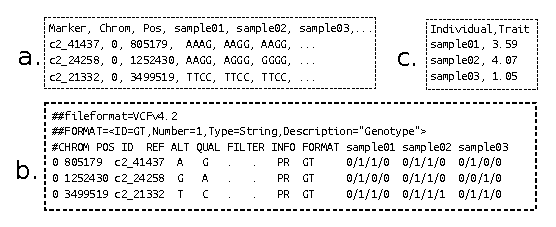
\includegraphics{images/paper-input-files}
\par\end{centering}
\caption{\scriptsize \textbf{{Examples of MultiGWAS input file formats}}. Figures a and b show genotype files in GWASpoly and VCF formats, respectively, while figure c shows a phenotype file in a matrix format. a. Genotype file in GWASpoly format containing column headers and with the first three columns for markers names, chromosomes, and positions. The following columns correspond to the marker data of the samples in \textquotedbl{}ACGT\textquotedbl{} format (e.g., AAGG, CCTT for tetraploids, AG, CT for diploids). b. Genotype file in VCF format with metadata (first two lines) and header line. The following lines contain genotype information of the samples for each position. VCF marker data can be encoded as simple genotype calls (GT format field, e.g., 0/0/1/1 for tetraploids or 0/1 for diploids) or using the NGSEP custom format fields (\cite{Duitama2019}): ACN, ADP or BSDP. c. Phenotype file in a matrix format with column headers and sample names followed by their trait values. Both GWASpoly genotype and phenotype files are in CSV (Comma Separated Values format).} \label{fig:File-Formats}\protect 
\end{figure}


\paragraph{GWAS model:}

MultiGWAS is designed to work with quantitative phenotypes and can run GWAS analysis using two types of statistical models that we have called \emph{full} and \emph{naive} models. The \emph{full model} is known in the literature as the Q+K model (\cite{Yu2006}) and includes a control for structure (Q) and relatedness between samples (K). In contrast, the \emph{naive model} does not include any type of correction. Both models are linear regression approaches, and each one of the four GWAS packages used in MultiGWAS has some variations of those models. The \emph{naive} is modeled with Generalized Linear Models (GLMs, Phenotype + Genotype), and the \emph{full} is modeled with Mixed Linear Models (MLMs, Phenotype + Genotype + Structure + Kinship). The default model used by MultiGWAS is the \emph{full model} (Q+K) (\cite{Yu2006}), following the equation:

\[
y=X\beta+S\alpha+Q\nu+Z\mu+e
\]

In this equation, the $y$ is the vector of observed phenotypes. Moreover, the $\beta$ is a vector of fixed effects other than SNP or population group effects, the $\alpha$ is a vector of SNP effects (Quantitative Trait Nucleotides), the $\nu$ is a vector of population effects, the $\mu$ is a vector of polygene background effects, and the $e$ is a vector of residual effects. Besides,  $Q$, modeled as a fixed effect, refers to the incidence matrix for subpopulation covariates relating $y$ to $\nu$, and $X$, $S$ and $Z$ are incidence matrices of 1s and 0s relating $y$ to $\beta$, $\alpha$ and $\mu$, respectively.


\paragraph{Genome-wide significance: }

GWAS searches SNPs associated with the phenotype in a statistically significant manner. A threshold or significance level $\alpha$ is specified and compared with the \emph{p-value} derived for each association score. Standard significance levels are 0.01 or 0.05 (\cite{Gumpinger2018,Rosyara2016}), and MultiGWAS uses an $\alpha$ of 0.05 for the four GWAS packages. However,  in GWASpoly and TASSEL, which calculates the SNP effect for each genotypic class using different gene action models (see ``Multi analysis stage''), the threshold is adjusted according to each of those two packages. Therefore, the number of tested markers\emph{ }may be different in each model (see below), impacting the \emph{p-value} thresholds.

\paragraph{Multiple testing correction:}

Due to the massive number of statistical tests performed by GWAS, it is necessary to perform a correction method for multiple hypothesis testing and adjusting the \emph{p-value} threshold accordingly. Two standard methods for multiple hypothesis testing are the false discovery rate (FDR) and the Bonferroni correction. The latter is the default method used by MultiGWAS, which is one of the most rigorous methods. However, instead of adjusting the \emph{p-values,} MultiGWAS adjust the threshold below which a \emph{p-value} is considered significant. That is $\alpha/m$, where $\alpha$ is the significance level and \emph{m }is the number of tested markers from the genotype matrix. 

\paragraph{Number of reported associations: }

Criticism has arisen, considering only statistically significant associations as possible correct associations (\cite{Thomson2011, Kaler2019}). Many low \emph{p-value} associations, closer to being significant, are discarded due to the stringent significance levels, which consequently increases the number of false negatives. To avoid this problem, MultiGWAS provides the option to specify the number of best-ranked associations (lower \emph{p-values}), adding the corresponding \emph{p-value} to each association found. In this way, it is possible to enlarge the number of results, and their replicability across the different programs. Nevertheless, the report displays each association with its corresponding \emph{p-value}.

%  We present the resultant associations in different tables and graphics reported by MultiGWAS (see Figure \ref{fig:-View-Shared-SNPs}). 

\paragraph{Quality control filters:}

A control step is necessary to check the input data for the genotype or phenotype errors or poor quality that can lead to spurious GWAS results. MultiGWAS provides the option to select and define thresholds for the following filters that control the data quality: Minor Allele Frequency (MAF), individual missing rate (MIND), SNP missing rate (GENO), and Hardy-Weinberg threshold (HWE):
\begin{itemize}
\item \textbf{MAF of }\textbf{\emph{x:}} filters out SNPs with minor allele frequency below \emph{x} (default 0.01); 
\item \textbf{MIND of }\textbf{\emph{x:}} filters out all individuals with missing genotypes exceeding \emph{x}{*}100\% (default 0.1); 
\item \textbf{GENO of }\textbf{\emph{x:}} filters out SNPs with missing values exceeding \emph{x}{*}100\% (default 0.1); 
\item \textbf{HWE of }\textbf{\emph{x:}} filters out SNPs with a \emph{p-value} below the \emph{x} threshold in the Hardy-Weinberg equilibrium exact test.(for diploids)

%\ic{Comentario de Andrés: una pregunta más metodológica tiene que ver con HWE. en poliploides la hetrocigosidad está inflada, y por ello desviaría en HWE si esté se calcula tradicionalmente. por ello, son las fercuencias genotípicas esperadas calculadas para poliplodes? i.e. (p+q) elevado a la n donde n es la ploidía}
\end{itemize}
MultiGWAS does the MAF filtering, and uses the PLINK package (\cite{Gumpinger2018}) for the other three filters: MIND, GENO, and HWE.

\paragraph{{GWAS tools:}}
List of names of the four GWAS software to run and integrate into MultiGWAS analysis. They are GWASpoly and SHEsis (designed for polyploid data), and PLINK and TASSEL (designed for diploid data). 

\subsubsection{Data preprocessing}

Once the configuration file is processed, the genomic data is read and cleaned by selecting individuals present in both genotype and phenotype. Then, MultiGWAS removes individuals and SNPs with poor quality following the previous selected quality-control filters and their thresholds, 

At this point, the format \textquotedbl{}ACGT\textquotedbl{} suitable for the polyploid software GWASpoly and SHEsis, is \textquotedbl{}diploidized\textquotedbl{} for PLINK and TASSEL. The homozygous tetraploid genotypes are converted to diploid thus: AAAA\textrightarrow AA, CCCC\textrightarrow CC, GGGG\textrightarrow GG, TTTT\textrightarrow TT. Moreover, for tetraploid heterozygous genotypes, the conversion depends on the reference and alternate alleles calculated for each position (e.g., AAAT \textrightarrow AT, ... ,CCCG\textrightarrow CG). 

After this process, MultiGWAS converts the genomic data, genotype, and phenotype datasets to the specific formats required for each of the four GWAS packages.
